\documentclass[12pt,a4paper]{report}
\usepackage[utf8]{inputenc}
\usepackage[T1]{fontenc}
\usepackage{geometry}
\geometry{margin=1in}
\usepackage{graphicx}
\usepackage{titlesec}
\usepackage{hyperref}
\usepackage{xcolor}
\usepackage{listings}
\usepackage{tikz}
\usetikzlibrary{shapes.geometric, arrows, positioning, calc, fit, backgrounds}
\usepackage{mdframed}
\usepackage{amsmath}
\usepackage{fancyhdr}

% Configure professional headers to match reference image
\setlength{\headheight}{14.5pt}
\addtolength{\topmargin}{-2.5pt}
\pagestyle{fancy}
\fancyhf{}
\fancyhead[L]{\itshape\leftmark}
\fancyhead[R]{\thepage}
\renewcommand{\headrulewidth}{0.4pt}
\renewcommand{\chaptermark}[1]{\markboth{Chapter \thechapter.\ #1}{}}

% Force headers on chapter start pages (usually 'plain' style)
\fancypagestyle{plain}{
  \fancyhf{}
  \fancyhead[L]{\itshape\leftmark}
  \fancyhead[R]{\thepage}
  \renewcommand{\headrulewidth}{0.4pt}
}

% Colors for the Mocha/Zoho theme
\definecolor{zoho-bg}{HTML}{1E1E2E}
\definecolor{zoho-blue}{HTML}{89B4FA}
\definecolor{zoho-green}{HTML}{A6E3A1}
\definecolor{zoho-red}{HTML}{F38BA8}
\definecolor{zoho-text}{HTML}{CDD6F4}

\hypersetup{
    colorlinks=true,
    linkcolor=zoho-blue,
    filecolor=magenta,      
    urlcolor=cyan,
    pdfpagemode=FullScreen,
    pdfnewwindow=true,
}

\title{Baseline kernel OS: Minimal 64-bit Microkernel}
\author{Atharva Bodade}
\date{May 2026}

\begin{document}

% --- 1. COVER PAGE ---
\begin{titlepage}
    \thispagestyle{empty}
    \begin{tikzpicture}[remember picture,overlay]
        \fill[zoho-bg!4] (current page.north west) rectangle ([yshift=-3.1cm]current page.north east);
        \fill[zoho-bg!2] (current page.south west) rectangle ([yshift=2.1cm]current page.south east);

        \draw[zoho-blue, line width=1.2pt] ([yshift=-3.15cm]current page.north west) -- ([yshift=-3.15cm]current page.north east);
        \draw[zoho-blue, line width=1.2pt] ([yshift=2.15cm]current page.south west) -- ([yshift=2.15cm]current page.south east);

        \node[anchor=north west, inner sep=0.75cm] at (current page.north west)
            {
\includegraphics[height=1.65cm]{docs/images/zoho_logo.png}};
        \node[anchor=north east, inner sep=0.75cm] at (current page.north east)
            {
\includegraphics[height=1.65cm]{docs/images/ssgmce_logo-removebg-preview.png}};
    \end{tikzpicture}

    \centering
    \vspace*{2.8cm}

    {\Huge\bfseries ZOHO SETU PROJECT \par}

    \vspace{1.25cm}
    {\small\color{zoho-blue}\textsc{Setu Project}} \par
    \vspace{0.35cm}
    \hrule height 1.1pt
    \vspace{0.75cm}
    {\Huge\bfseries Baseline kernel OS\par}
    \vspace{0.25cm}
    {\large\itshape Software Domain\par}
    \vspace{0.5cm}
    \hrule height 1.1pt

    \vspace{0.95cm}
    \begin{mdframed}[
        linecolor=zoho-blue,
        linewidth=1pt,
        backgroundcolor=white,
        roundcorner=10pt,
        innerleftmargin=16pt,
        innerrightmargin=16pt,
        innertopmargin=13pt,
        innerbottommargin=13pt
    ]
        \centering
        \textbf{Description}\par
        \vspace{0.3cm}
        Create a minimal 64-bit microkernel with core components like USB drivers, memory management, and a graphical shell.\par
        \vspace{0.5cm}
        \textbf{Project Type:} Linux \hspace{1.35cm} \textbf{Category:} Software Based
    \end{mdframed}

    \vspace{0.8cm}
    {\large\bfseries Atharva Bodade} \par
     \vspace{0.2cm}
    {\small Class: Third Year \par}
    \vspace{0.2cm}
    {\small Branch: Information Technology \par}
    \vspace{0.12cm}
    {\small Shri Sant Gajanan Maharaj College of Engineering, Shegaon \par}
    \vspace{0.25cm}
    {\small GitHub: \href{https://github.com/UnsettledAverage73/zoho-os}{https://github.com/UnsettledAverage73/zoho-os}} \par
    \vspace{0.2cm}
    {\small Presentation: \href{https://youtu.be/3w8XI3YLobc}{https://youtu.be/3w8XI3YLobc}} \par
    \vspace{0.2cm}
    {\small Reference: \href{https://kernel.org/}{https://kernel.org/}} \par

    \vfill
    {\large May 2026}
\end{titlepage}

\tableofcontents
\newpage

% --- 2. VISION \& PROBLEM STATEMENT ---
\chapter{Vision \& Problem Statement}
The goal of this project is to develop a minimal, educational Linux-type kernel from scratch. It serves as a baseline for understanding low-level systems programming, memory management, and driver development.

\section{The Limitations of Today}
Modern kernels like Linux are incredibly complex, making it difficult for students and researchers to grasp the core fundamentals of how an OS interacts with hardware. This project aims to strip away the complexity to provide a clear, functional baseline.

\section{Project Philosophy}
Baseline kernel OS is built to be a minimal yet extensible system. This requires:
\begin{itemize}
    \item \textbf{Educational Clarity:} Well-documented code that maps directly to architectural concepts.
    \item \textbf{Hardware Abstraction:} A clean interface between the kernel and the underlying x86\_64 hardware.
    \item \textbf{Extensibility:} A modular design that allows for easy addition of new drivers and system calls.
\end{itemize}

\newpage

% --- 3. ARCHITECTURE OVERVIEW ---
\chapter{Architecture Overview}
Baseline kernel OS implements a \textbf{Modular Monolithic Architecture}. While all core services run within the same address space in Ring 0 for performance, the system is logically divided into strictly defined layers and modules to ensure maintainability and structural clarity.

\section{System Architecture Diagram}
\begin{center}
\resizebox{0.95\textwidth}{!}{%
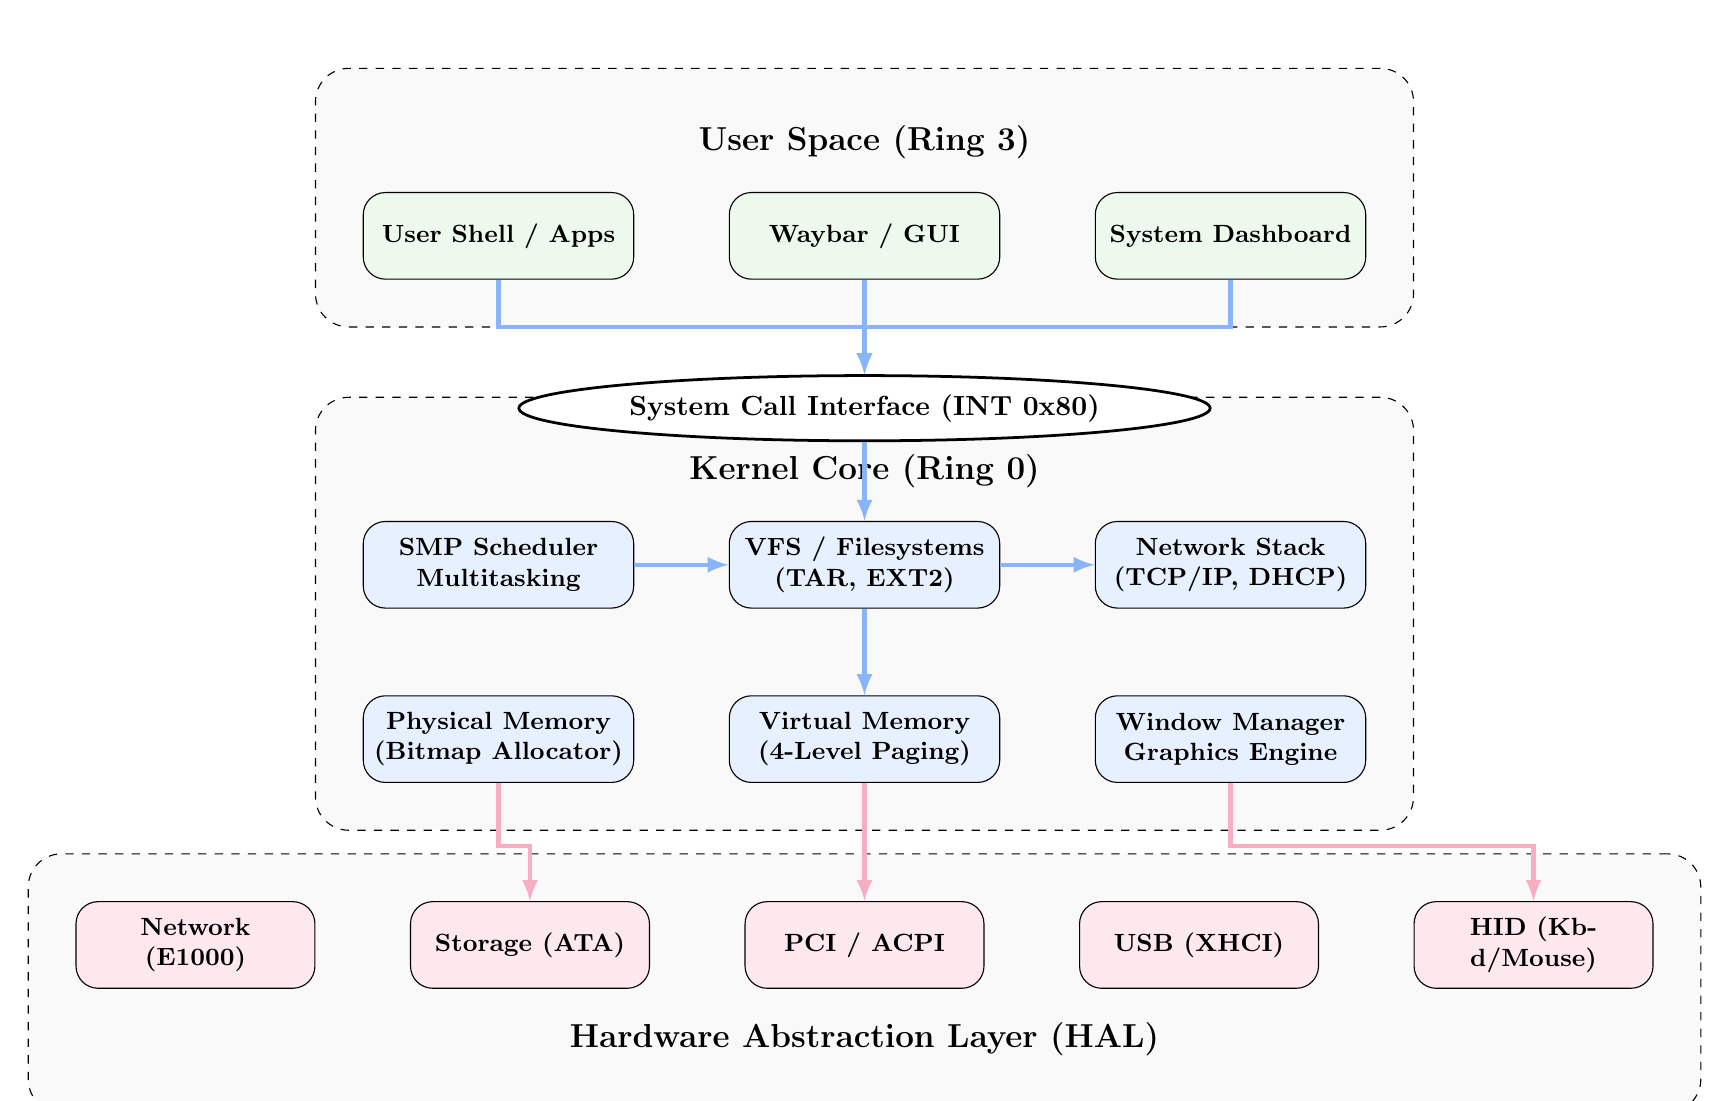
\begin{tikzpicture}[
    node distance=1.1cm and 1.2cm,
    layerbox/.style={draw, dashed, rounded corners=12pt, fill=gray!5, inner sep=0.6cm},
    usernode/.style={draw, rounded corners=8pt, fill=zoho-green!20, text width=3.2cm, text centered, minimum height=1.1cm, font=\small\bfseries},
    kernnode/.style={draw, rounded corners=8pt, fill=zoho-blue!20, text width=3.2cm, text centered, minimum height=1.1cm, font=\small\bfseries},
    hwnode/.style={draw, rounded corners=8pt, fill=zoho-red!20, text width=2.8cm, text centered, minimum height=1.1cm, font=\small\bfseries},
    link/.style={-latex, ultra thick, draw=zoho-blue},
    hwlink/.style={-latex, ultra thick, draw=zoho-red!70},
    note/.style={font=\large\bfseries}
]
    % --- Nodes Definitions ---
    % User Space (Ring 3)
    \node (gui) [usernode] {Waybar / GUI};
    \node (shell) [usernode, left=of gui] {User Shell / Apps};
    \node (stats) [usernode, right=of gui] {System Dashboard};
    \node (user_label) [note, above=0.3cm of gui] {User Space (Ring 3)};

    % System Call Interface
    \node (syscall) [draw, ellipse, fill=white, line width=1pt, below=1.2cm of gui, minimum width=7cm, minimum height=0.8cm] {\textbf{System Call Interface (INT 0x80)}};

    % Kernel Core (Ring 0)
    \node (vfs) [kernnode, below=1.0cm of syscall] {VFS / Filesystems\\(TAR, EXT2)};
    \node (sched) [kernnode, left=of vfs] {SMP Scheduler\\Multitasking};
    \node (net) [kernnode, right=of vfs] {Network Stack\\(TCP/IP, DHCP)};
    
    \node (vmm) [kernnode, below=of vfs] {Virtual Memory\\(4-Level Paging)};
    \node (pmm) [kernnode, left=of vmm] {Physical Memory\\(Bitmap Allocator)};
    \node (graphics) [kernnode, right=of vmm] {Window Manager\\Graphics Engine};
    \node (kern_label) [note, above=0.3cm of vfs] {Kernel Core (Ring 0)};

    % Hardware Abstraction Layer
    \node (pci) [hwnode, below=1.5cm of vmm] {PCI / ACPI};
    \node (storage) [hwnode, left=of pci] {Storage (ATA)};
    \node (nic) [hwnode, left=of storage] {Network (E1000)};
    \node (usb) [hwnode, right=of pci] {USB (XHCI)};
    \node (hid) [hwnode, right=of usb] {HID (Kbd/Mouse)};
    \node (hw_label) [note, below=0.3cm of pci] {Hardware Abstraction Layer (HAL)};

    % --- Background Boxes ---
    \begin{scope}[on background layer]
        \node (user_box) [layerbox, fit=(shell) (stats) (user_label)] {};
        \node (kern_box) [layerbox, fit=(sched) (net) (graphics) (pmm) (kern_label) (vfs)] {};
        \node (hw_box) [layerbox, fit=(pci) (hid) (nic) (hw_label)] {};
    \end{scope}

    % --- Connections ---
    \draw [link] (gui.south) -- (syscall.north);
    \draw [link] (shell.south) -- ++(0,-0.6) -| (syscall.north);
    \draw [link] (stats.south) -- ++(0,-0.6) -| (syscall.north);
    
    \draw [link] (syscall.south) -- (vfs.north);
    \draw [link] (vfs.south) -- (vmm.north);
    \draw [link] (sched.east) -- (vfs.west);
    \draw [link] (vfs.east) -- (net.west);
    
    \draw [hwlink] (vmm.south) -- (pci.north);
    \draw [hwlink] (pmm.south) -- ++(0,-0.8) -| (storage.north);
    \draw [hwlink] (graphics.south) -- ++(0,-0.8) -| (hid.north);

\end{tikzpicture}
}
\end{center}

\section{Structural Integrity}
The architecture is designed around three primary pillars:
\begin{itemize}
    \item \textbf{Isolation:} User-space applications are strictly isolated from the kernel and each other via 4-level paging and hardware-enforced protection rings.
    \item \textbf{Abstraction:} The VFS and HAL provide a consistent interface for higher-level systems, allowing hardware-specific details to be swapped or updated without affecting the core logic.
    \item \textbf{Observability:} Integrated logging (\texttt{klog}), statistics (\texttt{kstats}), and tracing (\texttt{ktrace}) are built into the kernel core to facilitate real-time debugging and performance monitoring.
\end{itemize}

\newpage

% --- 4. BOOT PROCESS ---
\chapter{Boot Process}
The transition from a powered-off state to a running 64-bit environment involves a complex handoff between assembly and C.

\section{System Lifecycle \& Boot Sequence}
The end-to-end initialization of Baseline kernel OS follows a strictly defined sequence of handoffs between hardware, firmware, and software layers.

\begin{center}
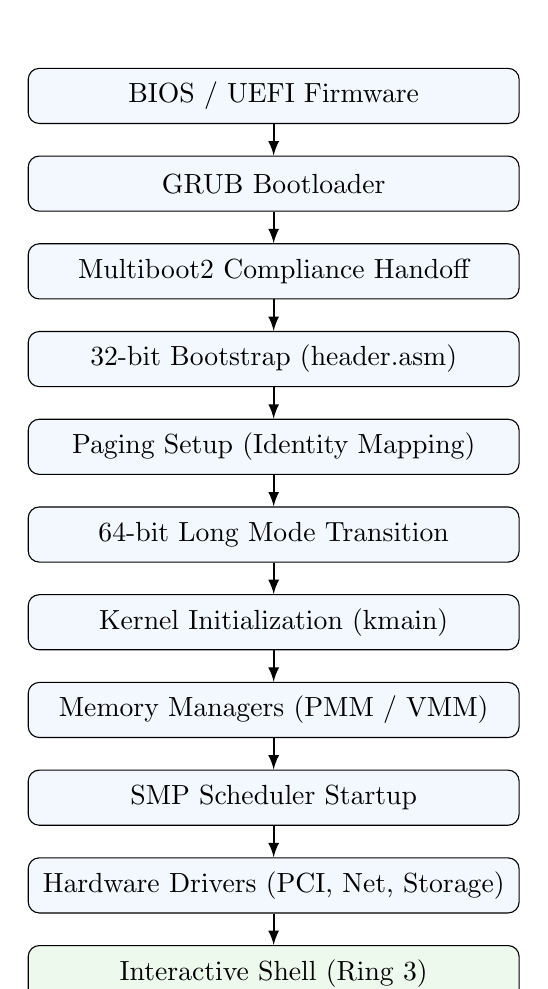
\begin{tikzpicture}[
    box/.style={draw, fill=zoho-blue!10, text width=6cm, text centered, minimum height=0.7cm, rounded corners},
    arrow/.style={-latex, thick}
]
    \node (1) [box] {BIOS / UEFI Firmware};
    \node (2) [box, below=0.4cm of 1] {GRUB Bootloader};
    \node (3) [box, below=0.4cm of 2] {Multiboot2 Compliance Handoff};
    \node (4) [box, below=0.4cm of 3] {32-bit Bootstrap (header.asm)};
    \node (5) [box, below=0.4cm of 4] {Paging Setup (Identity Mapping)};
    \node (6) [box, below=0.4cm of 5] {64-bit Long Mode Transition};
    \node (7) [box, below=0.4cm of 6] {Kernel Initialization (kmain)};
    \node (8) [box, below=0.4cm of 7] {Memory Managers (PMM / VMM)};
    \node (9) [box, below=0.4cm of 8] {SMP Scheduler Startup};
    \node (10) [box, below=0.4cm of 9] {Hardware Drivers (PCI, Net, Storage)};
    \node (11) [box, fill=zoho-green!20, below=0.4cm of 10] {Interactive Shell (Ring 3)};

    \draw [arrow] (1) -- (2);
    \draw [arrow] (2) -- (3);
    \draw [arrow] (3) -- (4);
    \draw [arrow] (4) -- (5);
    \draw [arrow] (5) -- (6);
    \draw [arrow] (6) -- (7);
    \draw [arrow] (7) -- (8);
    \draw [arrow] (8) -- (9);
    \draw [arrow] (9) -- (10);
    \draw [arrow] (10) -- (11);
\end{tikzpicture}
\end{center}

\section{Boot Sequence File Mapping}
The following table maps the logical stages of the boot process to their respective implementation files in the source tree.

\begin{table}[h]
\centering
\begin{tabular}{|l|l|p{6cm}|}
\hline
\textbf{Stage} & \textbf{Source File} & \textbf{Primary Responsibility} \\ \hline
Multiboot2 Header & \texttt{src/boot/header.asm} & GRUB handshake and 32-bit entry. \\ \hline
32-bit Bootstrap & \texttt{src/boot/main.asm} & Identity paging and GDT setup. \\ \hline
Long Mode Setup & \texttt{src/boot/main.asm} & CPU far jump and 64-bit transition. \\ \hline
Kernel Main & \texttt{src/kernel/main.c} & High-level C entry and initialization. \\ \hline
Memory Setup & \texttt{pmm.c / vmm.c} & Physical and virtual memory context. \\ \hline
SMP Handoff & \texttt{trampoline.asm} & AP (Application Processor) startup logic. \\ \hline
\end{tabular}
\caption{Boot Process File Mapping}
\end{table}

\section{Key Milestones}
\begin{enumerate}
    \item \textbf{Multiboot2 Header:} Allows GRUB to recognize the kernel.
    \item \textbf{PAE Paging:} Necessary to address the 64-bit space.
    \item \textbf{GDT Flush:} Loading the global descriptor table for code and data segments.
\end{enumerate}

\newpage

% --- 5. CORE KERNEL SYSTEMS ---
\chapter{Core Kernel Systems}

\section{Physical Memory Manager (PMM)}
The PMM uses a high-performance hybrid architecture, combining a stack-based frame allocator for $O(1)$ allocation with a bitmap tracker for validation and redundancy.

\begin{center}
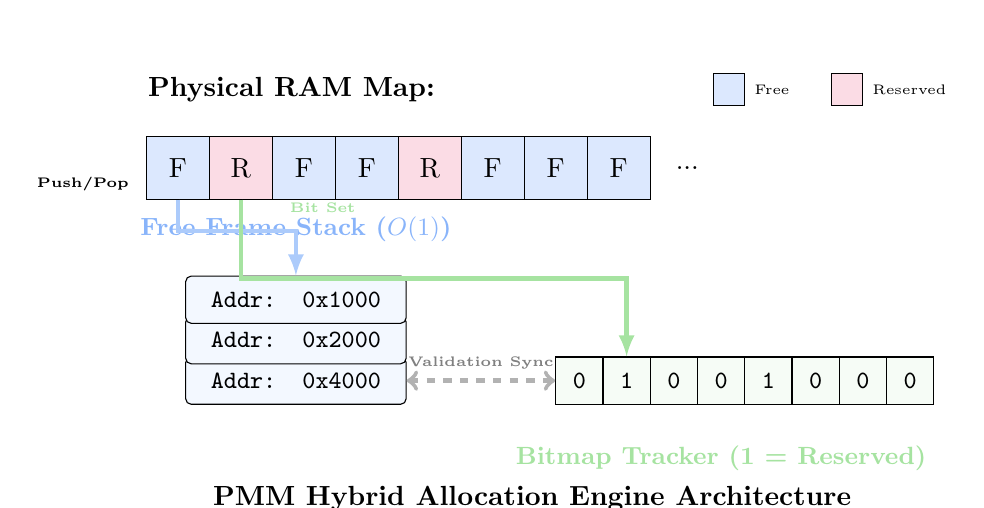
\begin{tikzpicture}[
    mem/.style={draw, fill=gray!10, minimum width=0.8cm, minimum height=0.8cm, outer sep=0pt},
    free/.style={fill=zoho-blue!30},
    used/.style={fill=zoho-red!30},
    stack/.style={draw, fill=zoho-blue!10, minimum width=2.8cm, minimum height=0.6cm, rounded corners=2pt, font=\small\ttfamily},
    bitmap/.style={draw, fill=zoho-green!10, minimum width=0.6cm, minimum height=0.6cm, font=\small\ttfamily},
    arrow/.style={-latex, ultra thick, draw=zoho-blue!70}
]
    % Physical RAM Map
    \node[anchor=west] at (-0.5, 3.2) {\textbf{Physical RAM Map:}};
    \foreach \x [count=\i] in {0,...,7} {
        \ifnum\i=2 \node (m\x) [mem, used] at (\x*0.8, 2.2) {R};
        \else \ifnum\i=5 \node (m\x) [mem, used] at (\x*0.8, 2.2) {R};
        \else \node (m\x) [mem, free] at (\x*0.8, 2.2) {F};
        \fi \fi
    }
    \node[right=0.2cm of m7] {...};

    % Legend (Moved higher)
    \node[mem, free, scale=0.5, label=right:{\tiny Free}] at (7, 3.2) {};
    \node[mem, used, scale=0.5, label=right:{\tiny Reserved}] at (8.5, 3.2) {};

    % Free Frame Stack (Adjusted Position)
    \node (s3) [stack] at (1.5, -0.5) {Addr: 0x4000};
    \node (s2) [stack, above=-0.1cm of s3] {Addr: 0x2000};
    \node (s1) [stack, above=-0.1cm of s2] {Addr: 0x1000};
    \node[above=0.3cm of s1, font=\bfseries\small, text=zoho-blue] {Free Frame Stack ($O(1)$)};
    
    % Bitmap Tracker (Adjusted Position)
    \foreach \b [count=\j] in {0,1,0,0,1,0,0,0} {
        \node (b\j) [bitmap] at (4.5 + \j*0.6, -0.5) {\b};
    }
    \node[below=0.4cm of b4, font=\bfseries\small, text=zoho-green] {Bitmap Tracker (1 = Reserved)};

    % Connections (Fixed Overlaps)
    \draw[arrow] (m0.south) -- ++(0,-0.4) -| (s1.north);
    \node[left=0.1cm of m0, yshift=-0.2cm, font=\tiny\bfseries] {Push/Pop};
        
    \draw[arrow, draw=zoho-green] (m1.south) -- ++(0,-1.0) -| (b2.north);
    \node[right=0.1cm of m1, yshift=-0.5cm, font=\tiny\bfseries, text=zoho-green] {Bit Set};
        
    \draw[<->, dashed, ultra thick, draw=gray!60] (s3.east) -- (b1.west) 
        node[midway, above, font=\tiny\bfseries, text=gray] {Validation Sync};

    \node at (4.5, -2.0) {\textbf{PMM Hybrid Allocation Engine Architecture}};
\end{tikzpicture}
\end{center}

\section{Virtual Memory Manager (VMM)}
Baseline kernel OS implements a 4-level paging system.
\begin{center}
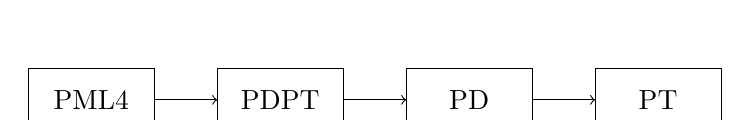
\begin{tikzpicture}[scale=0.8]
    \draw (0,0) rectangle (2,1) node[midway] {PML4};
    \draw (3,0) rectangle (5,1) node[midway] {PDPT};
    \draw (6,0) rectangle (8,1) node[midway] {PD};
    \draw (9,0) rectangle (11,1) node[midway] {PT};
    \draw[->] (2,0.5) -- (3,0.5);
    \draw[->] (5,0.5) -- (6,0.5);
    \draw[->] (8,0.5) -- (9,0.5);
\end{tikzpicture}
\end{center}
\section{Interrupt Handling \& IDT}
Baseline kernel OS manages hardware asynchronous events through a centralized Interrupt Descriptor Table (IDT).
\begin{center}
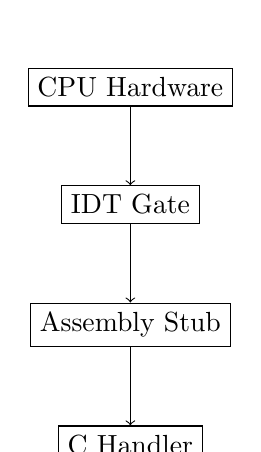
\begin{tikzpicture}[node distance=1cm, auto]
    \node (cpu) [draw] {CPU Hardware};
    \node (idt) [draw, below=of cpu] {IDT Gate};
    \node (stub) [draw, below=of idt] {Assembly Stub};
    \node (isr) [draw, below=of stub] {C Handler};
    \draw[->] (cpu) -- (idt);
    \draw[->] (idt) -- (stub);
    \draw[->] (stub) -- (isr);
\end{tikzpicture}
\end{center}

\section{SMP Scheduler \& Task Management}
The scheduler implements a multicore round-robin algorithm with per-CPU runqueues and task stealing for dynamic load balancing.

\begin{center}
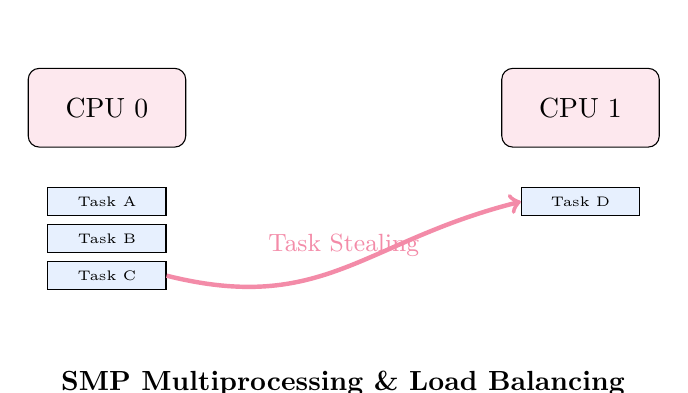
\begin{tikzpicture}[
    cpu/.style={draw, fill=zoho-red!20, minimum width=2cm, minimum height=1cm, rounded corners},
    task/.style={draw, fill=zoho-blue!20, minimum width=1.5cm, font=\tiny},
    link/.style={->, ultra thick}
]
    \node (cpu0) [cpu] {CPU 0};
    \node (cpu1) [cpu, right=4cm of cpu0] {CPU 1};
    
    \node (q0_1) [task, below=0.5cm of cpu0] {Task A};
    \node (q0_2) [task, below=0.1cm of q0_1] {Task B};
    \node (q0_3) [task, below=0.1cm of q0_2] {Task C};
    
    \node (q1_1) [task, below=0.5cm of cpu1] {Task D};
    
    \draw [link, zoho-red] (q0_3.east) .. controls +(2,-0.5) and +(-2,-0.5) .. (q1_1.west) 
        node[midway, above, font=\small] {Task Stealing};
        
    \node at (3,-3.5) {\textbf{SMP Multiprocessing \& Load Balancing}};
\end{tikzpicture}
\end{center}

\section{File System Design \& Data Flow}
The Baseline kernel OS filesystem is designed around a strictly hierarchical abstraction layer. This allows the kernel to treat hardware devices, local storage, and memory-backed archives through a unified "File" interface.

\begin{center}
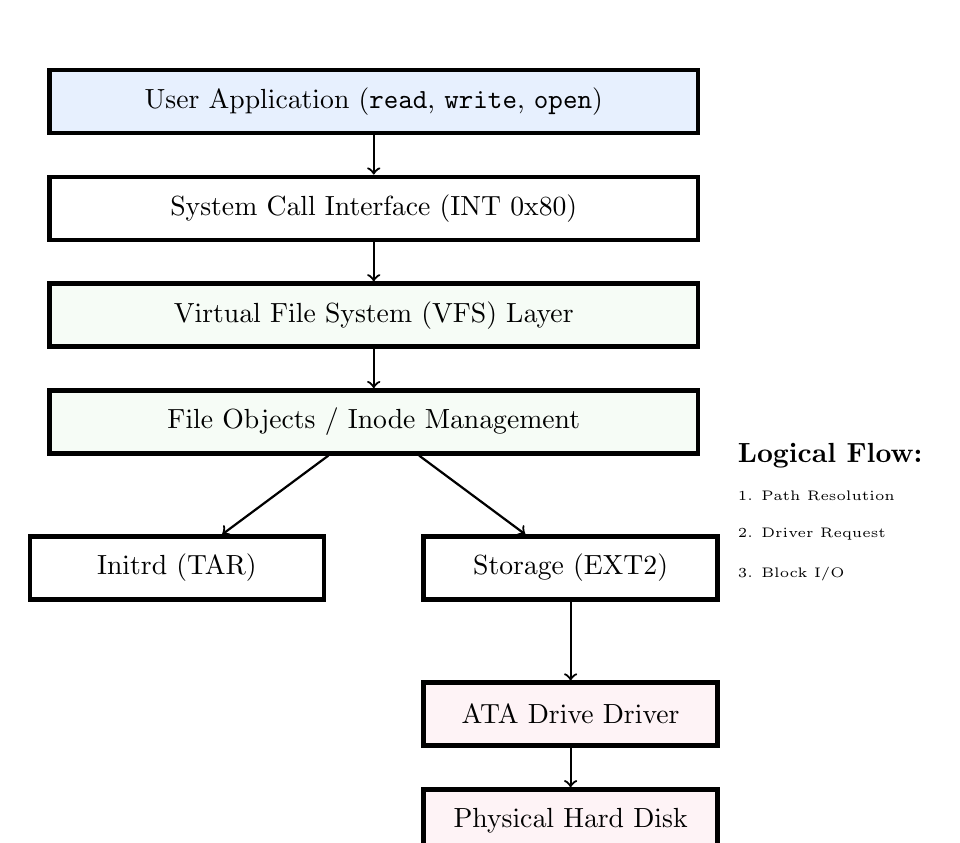
\begin{tikzpicture}[
    level/.style={draw, fill=white, text width=8cm, text centered, minimum height=0.8cm, ultra thick},
    api/.style={fill=zoho-blue!20},
    core/.style={fill=zoho-green!10},
    hw/.style={fill=zoho-red!10}
]
    \node (user) [level, api] {User Application (\texttt{read}, \texttt{write}, \texttt{open})};
    \node (syscall) [level, below=0.5cm of user] {System Call Interface (INT 0x80)};
    \node (vfs) [level, core, below=0.5cm of syscall] {Virtual File System (VFS) Layer};
    \node (obj) [level, core, below=0.5cm of vfs] {File Objects / Inode Management};
    
    \node (tar) [level, below=1cm of obj, xshift=-2.5cm, text width=3.5cm] {Initrd (TAR)};
    \node (ext2) [level, below=1cm of obj, xshift=2.5cm, text width=3.5cm] {Storage (EXT2)};
    
    \node (ata) [level, hw, below=1cm of ext2, text width=3.5cm] {ATA Drive Driver};
    \node (phys) [level, hw, below=0.5cm of ata, text width=3.5cm] {Physical Hard Disk};

    \draw [->, thick] (user) -- (syscall);
    \draw [->, thick] (syscall) -- (vfs);
    \draw [->, thick] (vfs) -- (obj);
    \draw [->, thick] (obj) -- (tar);
    \draw [->, thick] (obj) -- (ext2);
    \draw [->, thick] (ext2) -- (ata);
    \draw [->, thick] (ata) -- (phys);

    \node[anchor=west] at (4.5, -4.5) {\textbf{Logical Flow:}};
    \node[anchor=west, font=\tiny] at (4.5, -5.0) {1. Path Resolution};
    \node[anchor=west, font=\tiny] at (4.5, -5.5) {2. Driver Request};
    \node[anchor=west, font=\tiny] at (4.5, -6.0) {3. Block I/O};
\end{tikzpicture}
\end{center}

\section{Filesystem Implementation Mapping}
The hierarchical design of the VFS is implemented across the following modules:

\begin{table}[h]
\centering
\begin{tabular}{|l|l|p{6cm}|}
\hline
\textbf{Layer} & \textbf{Source File} & \textbf{Implementation Role} \\ \hline
VFS Abstraction & \texttt{src/kernel/vfs.c} & Path parsing and driver dispatching. \\ \hline
Initrd Driver & \texttt{src/kernel/tar.c} & Read-only access to disk-backed TAR archive. \\ \hline
Storage Driver & \texttt{src/kernel/ext2.c} & Ext2 block and inode management. \\ \hline
Block I/O & \texttt{src/kernel/ata.c} & Low-level ATA PIO mode disk driver. \\ \hline
Device Nodes & \texttt{src/kernel/tty.c} & Character device interface for \texttt{/dev/tty}. \\ \hline
\end{tabular}
\caption{Filesystem Implementation Mapping}
\end{table}

\begin{itemize}
    \item \textbf{Disk-backed TAR:} Used for the initial ramdisk and system applications.
    \item \textbf{Device Nodes:} Support for \texttt{/dev/tty} and \texttt{/dev/serial}.
\end{itemize}

\section{Observability (KStats \& KTrace)}
Baseline kernel OS includes built-in observability tools that track kernel performance from the earliest boot stages.
\begin{itemize}
    \item \textbf{KStats:} Monitors physical memory usage, uptime, and active task counts.
    \item \textbf{KTrace:} Provides an event buffer for high-speed tracing of kernel execution paths, essential for debugging race conditions in SMP mode.
\end{itemize}

\section{Terminal Abstraction (TTY)}
The TTY layer provides a unified interface for text-based communication, multiplexing output between the local VGA framebuffer and the remote Serial (COM1) port.

\begin{center}
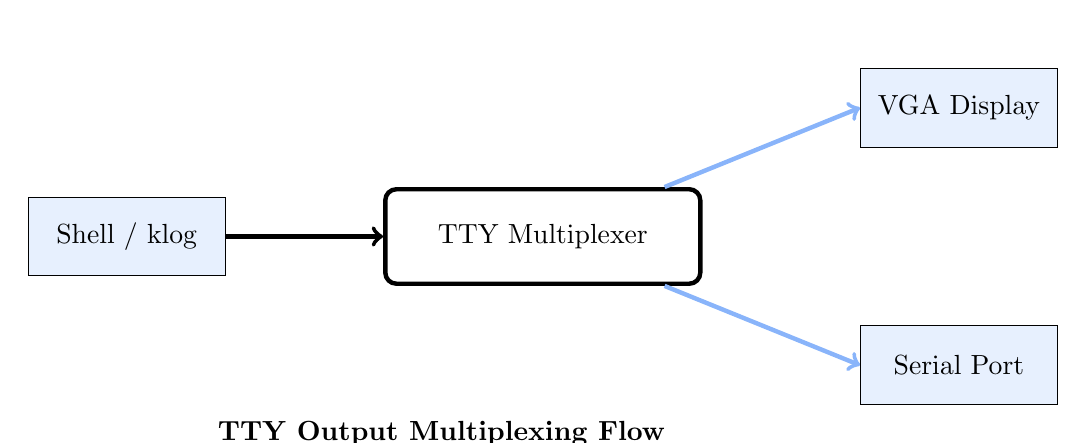
\begin{tikzpicture}[
    io/.style={draw, fill=zoho-blue!20, minimum width=2.5cm, minimum height=1cm},
    tty/.style={draw, fill=white, ultra thick, minimum width=4cm, minimum height=1.2cm, rounded corners}
]
    \node (shell) [io] {Shell / klog};
    \node (tty) [tty, right=2cm of shell] {TTY Multiplexer};
    \node (vga) [io, above right=0.5cm and 2cm of tty] {VGA Display};
    \node (serial) [io, below right=0.5cm and 2cm of tty] {Serial Port};
    
    \draw [->, ultra thick] (shell) -- (tty);
    \draw [->, ultra thick, zoho-blue] (tty) -- (vga.west);
    \draw [->, ultra thick, zoho-blue] (tty) -- (serial.west);
    
    \node at (4,-2.5) {\textbf{TTY Output Multiplexing Flow}};
\end{tikzpicture}
\end{center}

\section{USB Support (XHCI)}
Baseline kernel OS features an eXtensible Host Controller Interface (XHCI) driver foundation, enabling high-speed communication with USB 3.0 devices such as human interface devices (HID) and mass storage.

\chapter{Shell Commands \& Interaction}
Baseline kernel OS provides a comprehensive interactive shell for system management, debugging, and application execution. The following table details the primary commands available.

\begin{table}[h]
\centering
\begin{tabular}{|l|p{6cm}|l|}
\hline
\textbf{Command} & \textbf{Description} & \textbf{Context} \\ \hline
\texttt{help} & Displays the list of all available commands. & General \\ \hline
\texttt{monitor} & Real-time CPU usage, Memory (MB used/total), and Task count. & Observability \\ \hline
\texttt{top} & Lists all active tasks with ID, CPU affinity, Ticks, and State. & Task Mgmt \\ \hline
\texttt{net} & Displays MAC/IP addresses and Packet RX/TX counts. & Networking \\ \hline
\texttt{ls} & Lists all files and directories in the current VFS path. & Storage \\ \hline
\texttt{cat <file>} & Reads and prints the contents of a file to the terminal. & Storage \\ \hline
\texttt{write <f> <t>} & Writes a string of text to a specified file. & Storage \\ \hline
\texttt{exec <file>} & Loads and executes a binary file from the VFS. & Process \\ \hline
\texttt{heap} & Detailed statistics of the Slab/Heap memory allocator. & Memory \\ \hline
\texttt{free} & Displays the total count of free physical memory frames. & Memory \\ \hline
\texttt{locks} & Shows acquisition and contention stats for kernel spinlocks. & Debugging \\ \hline
\texttt{stress\_proc} & Initiates a "Process Storm" test to verify scheduler stability. & Stress Test \\ \hline
\texttt{clear} & Clears the terminal screen and resets the cursor. & General \\ \hline
\end{tabular}
\caption{Primary Shell Commands}
\end{table}

\section{Interaction Examples}
Baseline kernel OS shell supports various commands for deep-system inspection and control.

\begin{figure}[h]
    \centering
    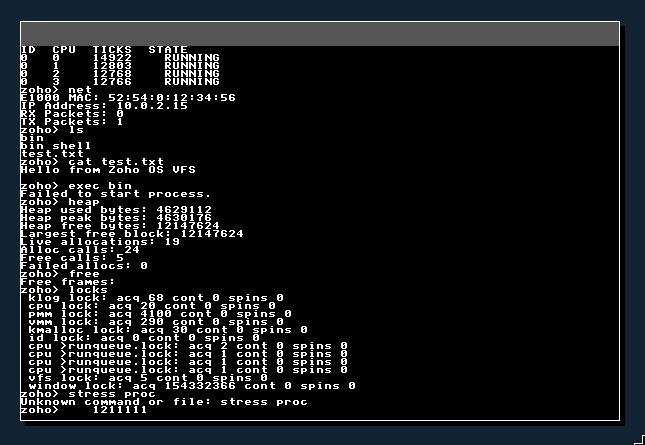
\includegraphics[width=0.9\textwidth]{docs/images/screenshot-2026-05-30_15-52-57.png}
    \caption{Shell Overview: Help system and core command execution.}
\end{figure}

\begin{figure}[h]
    \centering
    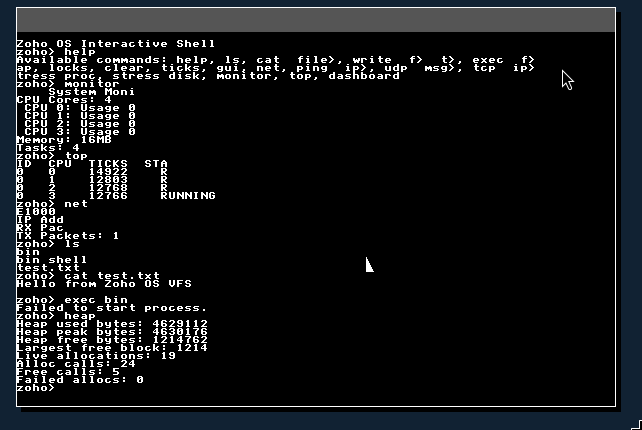
\includegraphics[width=0.9\textwidth]{docs/images/screenshot-2026-05-30_15-51-50.png}
    \caption{System Management: Task monitor and networking status.}
\end{figure}

\newpage
\textbf{System Telemetry (\texttt{monitor}):}
\begin{lstlisting}[basicstyle=\tiny, backgroundcolor=\color{gray!5}]
zoho> monitor
--- System Monitor ---
CPU Cores: 4
 CPU 0: Usage 12%
 CPU 1: Usage 5%
Memory: 24MB / 512MB used
Tasks: 8
\end{lstlisting}

\textbf{Task List (\texttt{top}):}
\begin{lstlisting}[basicstyle=\tiny, backgroundcolor=\color{gray!5}]
zoho> top
ID  CPU  TICKS  STATE
0   0    12500  RUNNING
1   1    450    READY
2   0    120    READY
\end{lstlisting}

\newpage
\chapter{Unique Features}
\section{Interactive Shell}
Baseline kernel OS features a userland shell that supports basic file operations and system queries.

\section{Video Demonstration \& Presentation}
A full demonstration of the Baseline kernel OS boot process, kernel initialization, and interactive shell, along with the project presentation, is available on YouTube.
\begin{center}
    \href{https://youtu.be/3w8XI3YLobc}{\Huge\textbf{[Watch the Project Presentation on YouTube]}}
\end{center}
\vspace{0.5cm}
\begin{center}
    \href{https://www.youtube.com/watch?v=gFLKEqt4GPs}{\Large\textbf{[Watch the Baseline kernel OS Demo on YouTube]}}
\end{center}

\section{Educational Video Series}
In addition to the core demonstration, a comprehensive tutorial series is available that documents the entire development lifecycle of the Baseline kernel OS. This series explains every technical term, architectural trade-off, and code implementation detail, serving as a primary educational resource for aspiring systems programmers.
\begin{center}
    \href{https://youtube.com/playlist?list=PLb1KzvlWYXQyj9d0_CZLnfdKmXT8Cd8uO&si=qObA4ucaPsYkwjuy}{\textbf{[Access the Full "Build OS from Scratch" Tutorial Series on YouTube]}}
\end{center}

\section{Real-time System Monitor}
The Dashboard task provides live CPU and Memory statistics. It runs as a separate kernel task, demonstrating the scheduler's ability to handle background observability.

\section{GUI Performance Optimization}
The window manager uses a "Dirty Rectangle" algorithm to minimize redraw overhead, combined with a dedicated kernel task to ensure smooth rendering even under heavy kernel load.

\newpage

% --- 7. TECHNICAL CHALLENGES ---
\chapter{Technical Challenges}

\section{Standardizing Framebuffer Pitch}
\textbf{Problem:} Initial graphics implementation resulted in a black screen or skewed output on certain virtualized hardware.
\textbf{Discovery:} I found that hardware often uses a `pitch` (bytes per scanline) that is wider than the visible width.
\textbf{Resolution:} Refactored all graphics primitives (\texttt{clear}, \texttt{blit}, \texttt{put\_pixel}) to use \texttt{fb\_pitch} for coordinate calculations instead of simple \texttt{width * 4}.

\section{The Huge Page Corruption Bug}
An \texttt{INT 6} fault occurred because the VMM treated 2MB Huge Pages as tables. 
\textbf{Resolution:} Refactored the identity map to use 4KB pages and updated VMM to handle flag propagation correctly. This ensures that 4KB mappings can coexist with the initial identity map without corrupting executable code.

\section{Memory Overlap (OOM)}
The heap and PMM were conflicting on the same physical range.
\textbf{Resolution:} Explicitly reserved the 128MB heap range in the PMM bitmap.

\newpage

% --- 8. FUTURE ROADMAP ---
\chapter{Future Roadmap}
Baseline kernel OS is envisioned as a continuously evolving platform for systems research and education. The following roadmap outlines the strategic technical goals categorized by implementation horizon.

\section{Short-Term: Stabilization \& Core I/O}
\begin{itemize}
    \item \textbf{Complete XHCI Driver}: Move beyond the initialization stub to support USB HID (Keyboards/Mice) and Mass Storage protocols via the XHCI controller.
    \item \textbf{FAT32 Filesystem Support}: Implement a read/write driver for FAT32 to enable interoperability with standard bootable media and easier data exchange.
    \item \textbf{Userspace Standard Library (libc)}: Develop a minimal C standard library to provide a stable API for userland application development, moving away from direct inline assembly syscalls.
\end{itemize}

\section{Mid-Term: Performance \& Compatibility}
\begin{itemize}
    \item \textbf{VirtIO Hardware Acceleration}: Implement VirtIO drivers for GPU and Network interfaces to achieve near-native performance in virtualized environments like QEMU and KVM.
    \item \textbf{Advanced Scheduling}: Transition the round-robin scheduler to a multi-level feedback queue (MLFQ) or a Completely Fair Scheduler (CFS) to better handle diverse workloads.
    \item \textbf{POSIX Signal Handling}: Implement a basic signal architecture to support standard process communication and exception handling in userland.
\end{itemize}

\section{Long-Term: Self-Hosting \& Distributed Systems}
\begin{itemize}
    \item \textbf{Self-Hosting Environment}: The ultimate milestone is to port a C compiler (like TCC or a minimal GCC) and an assembler to Baseline kernel OS, allowing the kernel to be recompiled from within itself.
    \item \textbf{Distributed Runtime for AI}: Research and implement a lightweight distributed memory architecture to support partitioned AI inference tasks across multiple network-linked OS instances.
    \item \textbf{Full Graphical Desktop Environment (DE)}: Expand the current window manager into a full-featured DE with a taskbar, file manager, and system settings suite.
\end{itemize}

\chapter{Setup \& Installation Guide}
Developing Baseline kernel OS requires a specific toolchain including a C compiler, assembler, and hardware emulator. This guide covers the installation process for major operating systems.

\section{Linux Environments}
Baseline kernel OS is natively developed on Linux. The following commands install the required dependencies (GCC, NASM, QEMU, GRUB, and Xorriso) for major distributions.

\subsection{Arch Linux}
\begin{lstlisting}[language=bash, basicstyle=\small\ttfamily, backgroundcolor=\color{gray!10}]
sudo pacman -S base-devel nasm qemu-desktop grub libisoburn mtools
\end{lstlisting}

\subsection{Debian / Ubuntu}
\begin{lstlisting}[language=bash, basicstyle=\small\ttfamily, backgroundcolor=\color{gray!10}]
sudo apt update
sudo apt install build-essential nasm qemu-system-x86 grub-pc-bin grub-common xorriso mtools
\end{lstlisting}

\subsection{RHEL / Fedora}
\begin{lstlisting}[language=bash, basicstyle=\small\ttfamily, backgroundcolor=\color{gray!10}]
sudo dnf groupinstall "Development Tools"
sudo dnf install nasm qemu-system-x86 grub2-tools xorriso mtools
\end{lstlisting}

\section{Windows Environment}
The recommended development environment for Windows users is **WSL2 (Windows Subsystem for Linux)**.

\begin{enumerate}
    \item \textbf{Install WSL2}: Open PowerShell as Administrator and run \texttt{wsl --install}.
    \item \textbf{Install Dependencies}: Once WSL is set up (Ubuntu is recommended), follow the \textbf{Debian / Ubuntu} instructions provided in the Linux section.
    \item \textbf{Graphical Output}: To view the OS GUI from WSL, ensure you are using Windows 11 with WSLg support, or install an X-Server like \textit{VcXsrv} or \textit{GWSL} on Windows 10.
\end{enumerate}

\section{Building and Running}
Once the environment is configured, use the following commands from the project root:
\begin{itemize}
    \item \textbf{Build ISO}: \texttt{make iso} - Compiles the kernel and generates a bootable \texttt{.iso} image.
    \item \textbf{Run in QEMU}: \texttt{make run} - Launches the OS in the QEMU emulator with multicore and XHCI support enabled.
\end{itemize}

\newpage

% --- 9. SCREENSHOTS / DEBUG LOGS ---
\chapter{System State}
\section{Terminal Output}
The following section provides real-time logs and visual confirmation of the Baseline kernel OS build and execution process.

\begin{figure}[h]
    \centering
    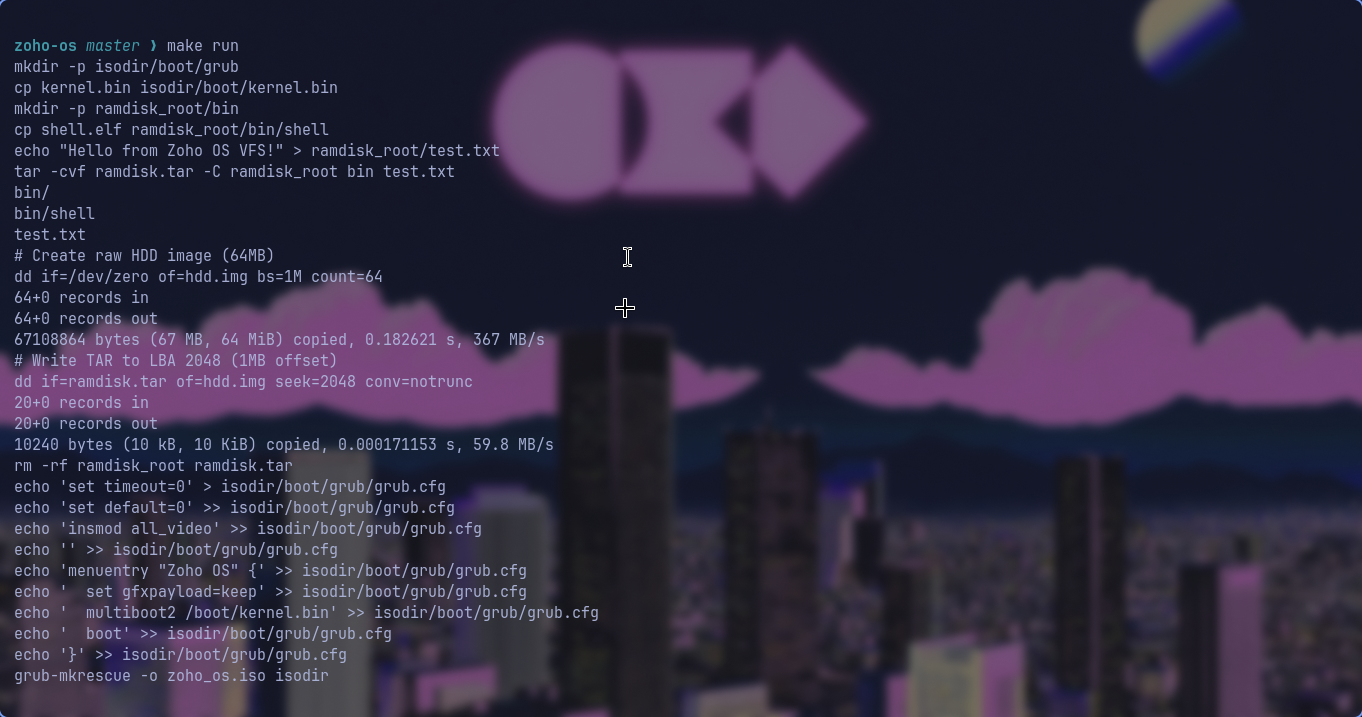
\includegraphics[width=0.9\textwidth]{docs/images/terminal_build.png}
    \caption{Build process and ISO generation via Makefile.}
\end{figure}

\begin{figure}[h]
    \centering
    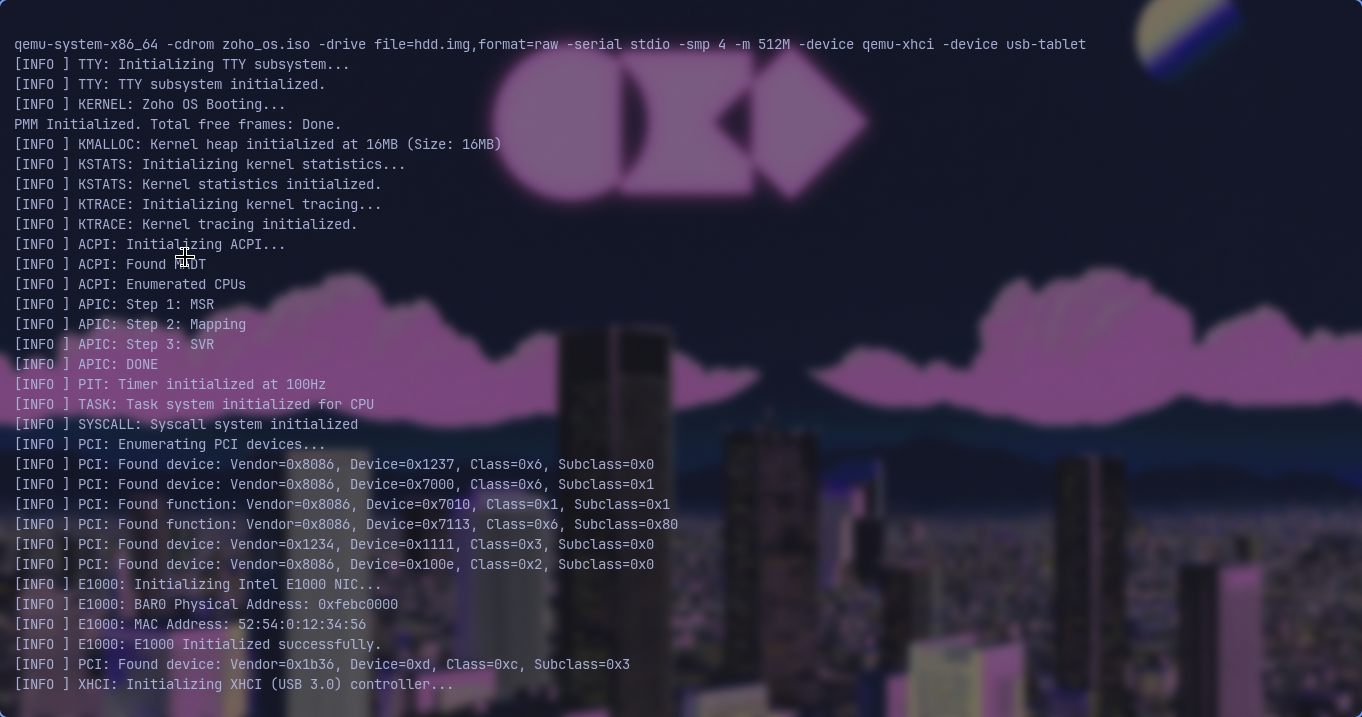
\includegraphics[width=0.9\textwidth]{docs/images/terminal_boot.png}
    \caption{Early kernel initialization and subsystem startup logs.}
\end{figure}

\begin{figure}[h]
    \centering
    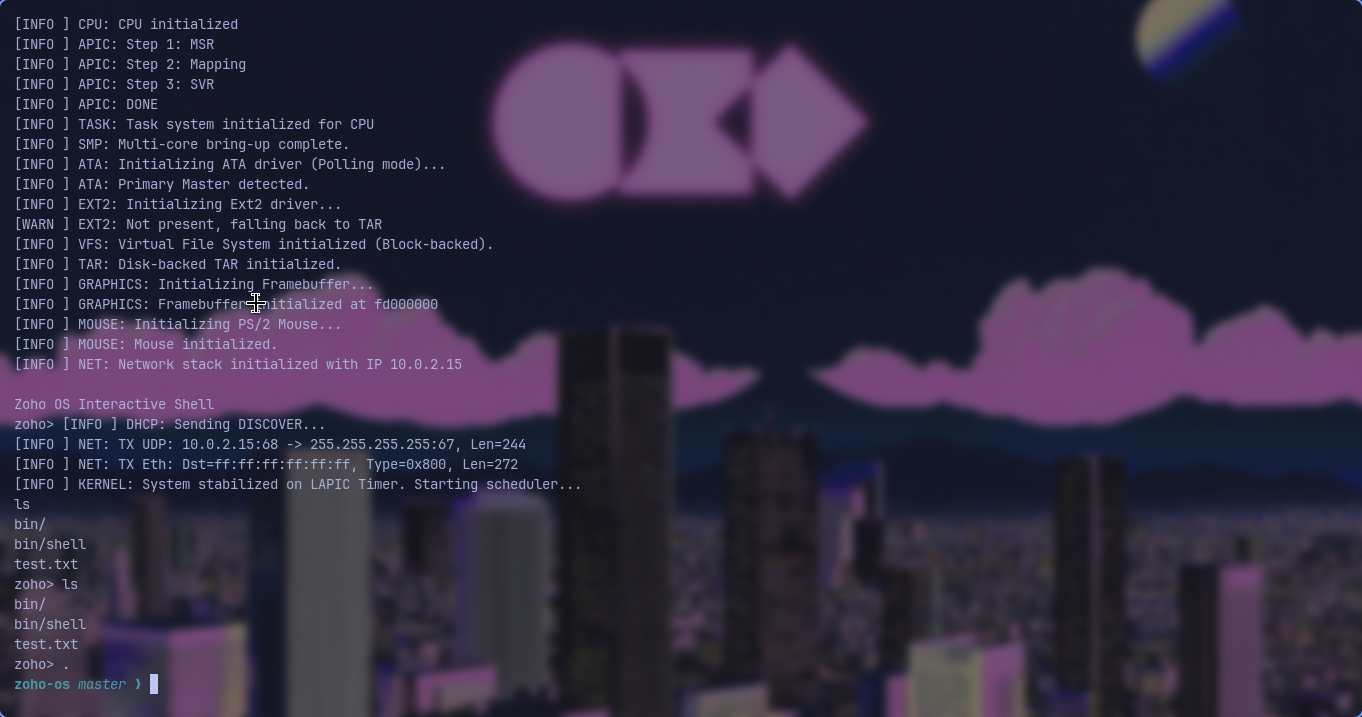
\includegraphics[width=0.9\textwidth]{docs/images/terminal_shell.png}
    \caption{Interactive shell session and final system stabilization.}
\end{figure}

\newpage
\section{Text-based Boot Logs}
\begin{lstlisting}[basicstyle=\tiny, backgroundcolor=\color{gray!10}]
[INFO ] TTY: Initializing TTY subsystem...
[INFO ] TTY: TTY subsystem initialized.
[INFO ] KERNEL: Baseline kernel OS Booting...
PMM Initialized. Total free frames: Done.
[INFO ] KMALLOC: Kernel heap initialized at 16MB (Size: 16MB)
[INFO ] KSTATS: Initializing kernel statistics...
[INFO ] KSTATS: Kernel statistics initialized.
[INFO ] KTRACE: Initializing kernel tracing...
[INFO ] KTRACE: Kernel tracing initialized.
[INFO ] ACPI: Initializing ACPI...
[INFO ] PCI: Enumerating PCI devices...
[INFO ] XHCI: Initializing XHCI (USB 3.0) controller...
[INFO ] XHCI: XHCI subsystem initialized (stub).
[INFO ] NET: Network stack initialized with IP 10.0.2.15

Baseline kernel OS Interactive Shell
zoho> ls
bin/
bin/shell
test.txt
\end{lstlisting}

\newpage

% --- 10. CONCLUSION ---
\chapter{Conclusion}
The development of \textbf{Baseline kernel OS} has been a comprehensive journey through the fundamental layers of modern computing. By stripping away the overwhelming complexity of production-grade kernels while retaining modern architectural paradigms, this project has successfully established a clear, functional baseline for 64-bit system development.

\begin{center}
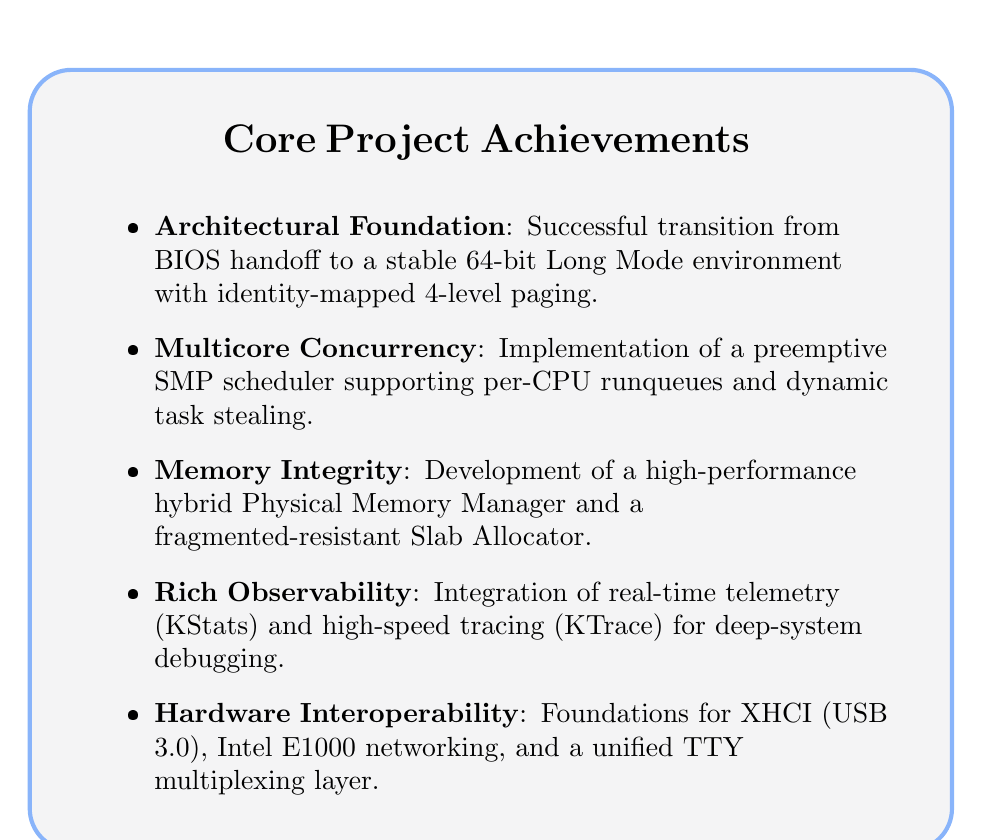
\begin{tikzpicture}
    \node (box) [draw, fill=zoho-bg!5, rounded corners=15pt, line width=1.5pt, draw=zoho-blue, text width=0.85\textwidth, inner sep=20pt] {
        \centering \Large \textbf{Core Project Achievements} \vspace{10pt}
        \normalsize
        \begin{itemize}
            \item \textbf{Architectural Foundation}: Successful transition from BIOS handoff to a stable 64-bit Long Mode environment with identity-mapped 4-level paging.
            \item \textbf{Multicore Concurrency}: Implementation of a preemptive SMP scheduler supporting per-CPU runqueues and dynamic task stealing.
            \item \textbf{Memory Integrity}: Development of a high-performance hybrid Physical Memory Manager and a fragmented-resistant Slab Allocator.
            \item \textbf{Rich Observability}: Integration of real-time telemetry (KStats) and high-speed tracing (KTrace) for deep-system debugging.
            \item \textbf{Hardware Interoperability}: Foundations for XHCI (USB 3.0), Intel E1000 networking, and a unified TTY multiplexing layer.
        \end{itemize}
    };
\end{tikzpicture}
\end{center}

\vspace{1cm}

Baseline kernel OS is more than just a proof-of-concept; it is a modular research platform designed for extensibility. The project achieves its educational mission by providing a transparent mapping between theoretical OS concepts and their low-level C and Assembly implementations. As outlined in the roadmap, the future of the project lies in achieving self-hosting status and exploring distributed AI runtimes, continuing the pursuit of efficient and observable system design.

\newpage

% --- 11. RESEARCH & REFERENCES ---
\chapter{Research \& References}
The development of Baseline kernel OS was informed by extensive research into x86\_64 architecture, low-level systems programming, and modern kernel design paradigms. The following resources served as primary technical references.

\begin{enumerate}
    \item \textbf{OSDev Wiki Contributors.} (2026). \textit{OSDev Wiki: The primary resource for OS development}. Available at: \href{https://wiki.osdev.org/}{https://wiki.osdev.org/}
    \item \textbf{Intel Corporation.} (2026). \textit{Intel 64 and IA-32 Architectures Software Developer’s Manual, Volume 3: System Programming Guide}. Available at: \href{https://software.intel.com/content/www/us/en/develop/articles/intel-sdm.html}{Intel SDM}
    \item \textbf{GNU Project.} (2026). \textit{Multiboot2 Specification, version 2.0}. Available at: \href{https://www.gnu.org/software/grub/manual/multiboot2/}{GNU.org}
    \item \textbf{UEFI Forum.} (2026). \textit{Advanced Configuration and Power Interface (ACPI) Specification, Revision 6.4}. Available at: \href{https://uefi.org/specifications}{UEFI.org}
    \item \textbf{Intel Corporation.} (2026). \textit{eXtensible Host Controller Interface (xHCI) for Universal Serial Bus, Revision 1.2}. Available at: \href{https://www.intel.com/content/www/us/en/io/universal-serial-bus/extensible-host-controler-interface-usb-xhci.html}{Intel xHCI Spec}
    \item \textbf{PCI-SIG.} (2026). \textit{PCI Local Bus Specification, Revision 3.0}. Available at: \href{https://pcisig.com/specifications}{PCI-SIG.com}
    \item \textbf{Torvalds, L., et al.} (2026). \textit{Linux Kernel Source Tree}. Available at: \href{https://github.com/torvalds/linux}{Linux Github}
\end{enumerate}

\newpage

% --- 11. FINAL PAGE ---
\chapter*{Contact \& Links}
\centering
\vspace{2cm}
\textbf{Atharva Bodade}\\
\vspace{1cm}
\href{mailto:atharvabodade@gmail.com}{atharvabodade@gmail.com}\\
\vspace{0.3cm}
\href{mailto:ssgm_308217@ssgmce.ac.in}{ssgm\_308217@ssgmce.ac.in}\\
\vspace{0.5cm}
\href{https://github.com/UnsettledAverage73}{GitHub Profile}\\
\vspace{0.3cm}
\href{https://www.linkedin.com/in/unsettledaverage73/}{LinkedIn Profile}\\
\vspace{0.3cm}
\href{https://youtu.be/3w8XI3YLobc}{Project Presentation}\\
\vspace{0.3cm}
\href{https://kernel.org/}{Project Reference}\\

\end{document}
